%================================================================
\section{Project plan}\label{sec:project_plan}
%================================================================
\begin{enumerate}
    \item Decide on theoretical background, such as articles and machine learning methods.
    \item Decide on environment setup and find experimental data with the same setup.
    \item Generate synthetic data using \verb|RatInABox| \cite{george:2022:ratinabox}
    \item Set up vanilla RNN using \verb|PyTorch| \cite{2017:pytorch}, and experiment with parameters.
    \item Expand experiment to include objects in the environment, and train the model to recognize these.
\end{enumerate}


%================================================================
\section{Progress report}\label{sec:progress_report}
%================================================================
I started researching path integration and the use of neural networks. Add something about choice of literature...

Decided on package to simulate data, and experimented with environment setup and generating trajectories. Figured out how to generate and combine these into dataset.

Did some tests using a basic RNN from PyTorch, which was not able to learn the correct path. Built a vanilla RNN using the module class provided by PyTorch. Got the model to make predictions similar to the generated trajectories, when taking time steps into account. So far I have tested the RNN using a hidden layer with 7 and 10 nodes, increasing number of nodes makes the predicted paths overlap the original ones. Did also test with different number of epochs, batch sizes and learning rates during implementation. Figure \ref{fig:test_model} shows model predictions, where none of the trajectories overlap the true ones.
\begin{figure}[H]
    \centering
    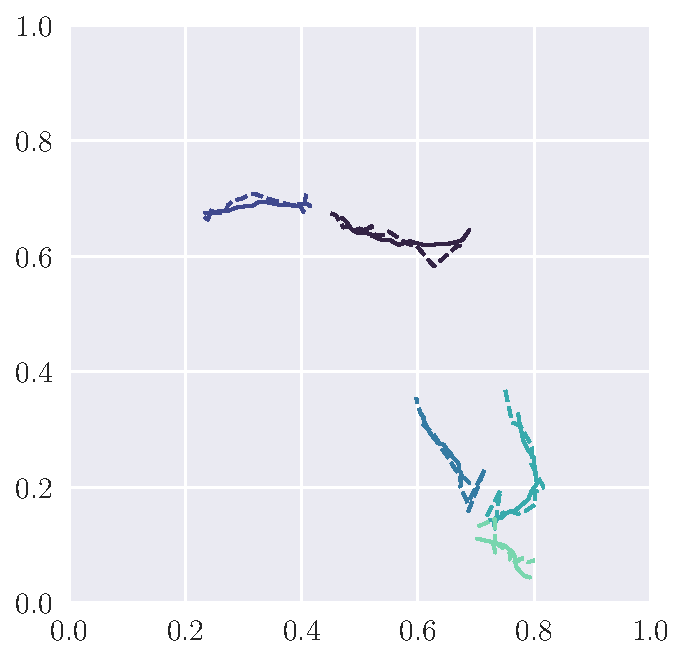
\includegraphics[width=\linewidth]{project/latex/figures/test_model.pdf}
    \caption{Predicted trajectories in dashed lines, and labels in full lines. 5 different sequences, consisting of 19 time steps.}
    \label{fig:test_model}
\end{figure}


%================================================================
\section{Future work}\label{sec:future_work}
%================================================================
Next step is to set up an experiment using both train and test set, where I collect data during both training and testing. I will also investigate different parameters such as learning rate and optimizers. In addition, I will compare the model performance using simulated and experimental data, using Sargollini data.